\section{Preferences}


\subsection{Consumer Preferences}

\slide{Consumer Preferences}{
    So far, the discussion has focused on \emph{what the consumer can afford}.
    Now, the focus of the discussion will shift towards \emph{what the consumer wants}.

    In order to do this, consumer preferences need to be studied.

    The end goal of consumer theory and optimisation is to find how to derive maximum satisfaction,
    given the consumer's constraints.
    
    The topic of `Budget Constraint' focuses on the `consumer's constraints' part.
    Now, the discussion will move towards `how to derive maximum satisfaction'.
}


\slide{Consumer Preferences}{
    Suppose two goods exist in an economy; good 1 and good 2.

    We create two bundles \(X = (x_1, x_2)\) and \(Y = (y_1, y_2)\).

    \begin{itemize}
        \item We say the consumer \textbf{strictly prefers} bundle X to Y and write:
        \[(x_1, x_2) \succ (y_1, y_2)\]
        \item We say the consumer \textbf{weakly prefers} bundle X to Y and write:
        \[(x_1, x_2) \succeq (y_1, y_2)\]
        \item We say the consumer is \textbf{indifferent} between bundles X \& Y and write:
        \[(x_1, x_2) \sim (y_1, y_2)\]
    \end{itemize}
}


\subsection{Assumptions}

\slide{Assumptions (Axioms)}{
\begin{itemize}
    \item We assume that preferences are \textbf{complete}. This means that given any two
    bundles in the budget set, the consumer has a preference.
    \begin{itemize}
        \item For any two bundles either \((x_1, x_2) \succ (y_1, y_2)\) or \((x_1, x_2) \succeq (y_1, y_2)\)
        or both i.e. \((x_1, x_2) \sim (y_1, y_2)\).
    \end{itemize}

    \item We assume that preferences are \textbf{reflexive}. This means that any bundle is
    at least as good as itself.
    \begin{itemize}
        \item For any bundle \((x_1, x_2) \succeq (y_1, y_2)\).
    \end{itemize}

    \item We assume that preferences are \textbf{transitive}. This means that if bundle A is preferred
    to B, and B is preferred to C, then A is preferred to C.
    \begin{itemize}
        \item For any three bundles X, Y, and Z: \((x_1, x_2) \succeq (y_1, y_2)\) and \((y_1, y_2) \succeq (z_1, z_2)\)
        implies \((x_1, x_2) \succeq (z_1, z_2)\).
    \end{itemize}
\end{itemize}
}



\section{Indifference Curves}


\subsection{Indifference Curves}

\slide{Indifference Curves}{
    Suppose we pick an arbitrary bundle X (\(x_1, x_2\)).

    \dfn{Indifference curve is the set of all bundles that the consumer is indifferent between.
    In essence, the bundles that the consumer likes as much as \((x_1, x_2)\) make up the indifference curve.}

    An indifference curve is the representation of a consumer's preferences. Therefore, it
    must obey completeness, reflexivity, and transitivity.

    Then, all bundles that are weakly preferred to \((x_1, x_2)\) form the \\ \textbf{weakly preferred set}.
    We can then say that the indifference curve forms the boundary to the weakly preferred
    set of a bundle.
}


\slide{Indifference Curves Graphically}{
\begin{center}
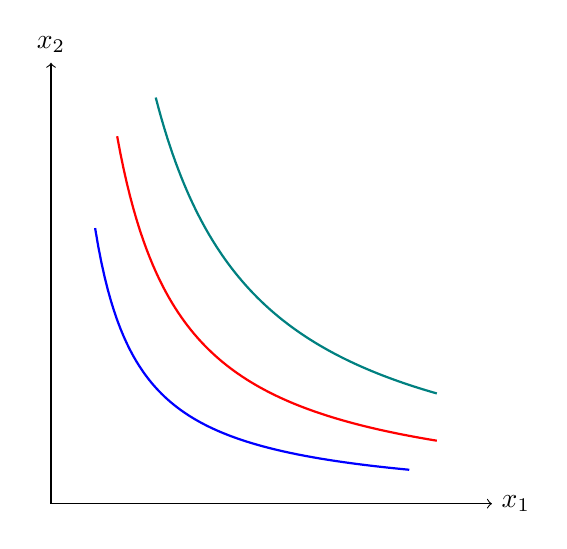
\begin{tikzpicture}[scale=0.7]
% Axes
\draw[->] (0,0) -- (8,0) node[right] {$x_1$};
\draw[->] (0,0) -- (0,8) node[above] {$x_2$};

% Indifference curve (example: x1 * x2 = 4  =>  x2 = 4/x1)
\draw[blue, thick, domain=0.8:6.5, samples=100]
    plot (\x, {4/\x});

\draw[red, thick, domain=1.2:7, samples=100]
    plot (\x, {8/\x});

\draw[teal, thick, domain=1.9:7, samples=100]
    plot (\x, {14/\x});
\end{tikzpicture}
\end{center}
}


\slide{Weakly Preferred Set}{
\begin{center}
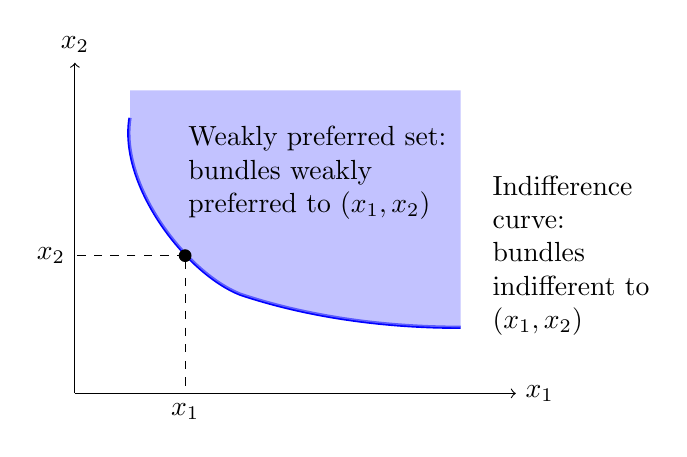
\begin{tikzpicture}[scale=0.7]

% Axes
\draw[->] (0,0) -- (8,0) node[right] {$x_1$};
\draw[->] (0,0) -- (0,6) node[above] {$x_2$};

% Indifference curve
\draw[very thick, blue]
    (1,5) .. controls (0.8,3.8) and (2,2.2) ..
    (3,1.8) .. controls (4.5,1.3) and (6,1.2) ..
    (7,1.2);

% Shaded weakly preferred set (area above curve)
\fill[blue!40, opacity=0.6]
    (1,5) 
    .. controls (0.8,3.8) and (2,2.2) ..
    (3,1.8) 
    .. controls (4.5,1.3) and (6,1.2) ..
    (7,1.2)
    -- (7,5.5)
    -- (1,5.5)
    -- cycle;

% Point (x1, x2)
\filldraw[black] (2,2.5) circle (3pt);

% Dashed projection lines
\draw[dashed] (2,2.4) -- (2,0);
\draw[dashed] (2,2.5) -- (0,2.5);

% Axis point labels
\node[below] at (2,0) {$x_1$};
\node[left] at (0,2.5) {$x_2$};

% Text annotations
\node[align=left] at (4.4,4)
{Weakly preferred set:\\
bundles weakly\\
preferred to $(x_1,x_2)$};

\node[align=left] at (9,2.5)
{Indifference\\
curve:\\
bundles\\
indifferent to\\
$(x_1,x_2)$};

\end{tikzpicture}
\end{center}
}


\slide{Indifference Curves Never Cross}{
    We require that indifference curves never cross. Why?

    \begin{center}
    \begin{tikzpicture}[scale=0.8]
    % Axes
    \draw[->] (0,0) -- (6,0) node[right] {$x_1$};
    \draw[->] (0,0) -- (0,6) node[above] {$x_2$};

    % First indifference curve: x1
    \draw[red, thick, domain=0.8:3.5, samples=100]
        plot (\x, {4/\x - 1});
        \filldraw[black] (1.05,2.8) circle (2pt);
        \node[above right] at (1.05,2.9) {$B$};

    % Second indifference curve: x2
    \draw[blue, thick, domain=0.5:5]
        plot (\x, {2/\x});
        \filldraw[black] (0.7,2.9) circle (2pt);
        \node[above right] at (-0.15,2.8) {$A$};

    \filldraw[black] (2,1) circle (2pt);
    \node[above right] at (2,1) {$C$};
    \end{tikzpicture}
    \end{center}
}

\slide{Indifference Curves Never Cross}{
    In the previous diagram, bundle B is in the weakly preferred set of bundle A. Therefore,
    the consumer (weakly) prefers bundle B to A.

    Furthermore, the consumer is indifferent between bundle A and C because they lie
    on the same indifference curve.

    However, the consumer is also indifferent between bundle C and B as they lie
    on the same indifference curve. By transitivity, if \(A \sim C\) and \(C \sim B\),
    it must be true that \(A \sim B\).

    There is a contradiction. This is why two indifference curves must not intersect.
}